\documentclass[9pt,twocolumn,twoside]{pnas-new}
% Use the lineno option to display guide line numbers if required.
%\usepackage{xcolor}
\templatetype{pnasresearcharticle} % Choose template
% {pnasresearcharticle} = Template for a two-column research article
% {pnasmathematics} %= Template for a one-column mathematics article
% {pnasinvited} %= Template for a PNAS invited submission

\begin{document}

%\title{Carbon sequestration trade-off between carbon assimilation and carbon losses through respiration and disturbances}
\title{Tradeoffs between carbon assimilation and release reveal a key role of the tropics in long-term global-scale carbon sequestration}

% Use letters for affiliations, numbers to show equal authorship (if applicable) and to indicate the corresponding author
\author[a,b,1]{Estefanía Muñoz}
\author[c]{Holger Metzler}
\author[a]{Marcos Fernández-Martínez}
\author[b]{Jacob A. Nelson}
\author[d]{Michael O'Sullivan}
\author[d]{Stephen Sitch}
\author[c]{Tobias Nützel}
\author[e]{Jens Heinke}
\author[f]{George Hurtt}
\author[f]{Lei Ma}
\author[g,h,i]{Qing Sun}
\author[j]{Patrick C. McGuire}
\author[k]{Etsushi Kato}
\author[l]{Xiaojuan Yang}
\author[m]{Wenping Yuan}
\author[b]{Carlos A. Sierra}

\affil[a]{CREAF, Cerdanyola del Vallès, Barcelona, Catalonia, Spain}
\affil[b]{Max Planck Institute for Biogeochemistry, Jena, Germany}
\affil[c]{Department of Geography, Ludwig-Maximilians-Universität in Munich, Munich, Germany}
\affil[d]{Faculty of Environment, Science and Economy, University of Exeter, Exeter, UK}
\affil[e]{Potsdam Institute for Climate Impact Research (PIK), Leibniz Association, P.O. Box 60 12 03, 14412 Potsdam, Germany}
\affil[f]{Department of Geographical Sciences, University of Maryland, College Park, MD 20770, USA}
\affil[g]{Climate and Environmental Physics, Physics Institute, University of Bern, Bern, Switzerland}
\affil[h]{Wyss Academy for Nature, University of Bern, Bern, Switzerland}
\affil[i]{Oeschger Centre for Climate Change Research, University of Bern, Bern, Switzerland}
\affil[j]{Department of Meteorology \& National Centre for Atmospheric Science (NCAS), University of Reading, Reading, United Kingdom}
\affil[k]{Institute of Applied Energy, Minato, Tokyo 105-0003, Japan}
\affil[l]{Environmental Sciences Division, Oak Ridge National Lab, Oak Ridge, TN 37830, USA}
\affil[m]{Institute of Carbon Neutrality, Sino-French Institute for Earth System Science, College of Urban and Environmental Sciences, Peking University, Beijing 100091, China}


% Please give the surname of the lead author for the running footer
\leadauthor{Muñoz et al.}

% Please add a significance statement to explain the relevance of your work
% Authors must submit a 120-word maximum statement about the significance of their research paper written at a level understandable to an undergraduate educated scientist outside their field of speciality. The primary goal of the significance statement is to explain the relevance of the work in broad context to a broad readership. The significance statement appears in the paper itself and is required for all research papers.
\significancestatement{Understanding terrestrial ecosystems' role in carbon sequestration is crucial for addressing global warming. This study provides key insights by analyzing carbon dynamics across time scales and latitudes, incorporating both natural processes and human-induced disturbances. By comparing various models and data products, we reveal that tropical regions show higher carbon sequestration potential when considering only assimilation and respiration; however, including disturbances shifts this advantage to higher latitudes, creating a substantial carbon debt in the tropics. These findings highlight the substantial carbon debt accumulated since pre-industrial times due to global disturbances, while suggesting untapped sequestration potential, particularly in tropical ecosystems. Our research emphasizes the importance of comprehensive, long-term assessments in developing effective climate mitigation strategies. It underscores the need for targeted conservation efforts to maximize the carbon sequestration capacity of terrestrial ecosystems worldwide.}

% Please include corresponding author, author contribution and author declaration information
\authorcontributions{CRediT Taxonomy of author contributions as follows. Conceptualization: EM, HM, CAS; Data Curation: EM, CAS; Formal Analysis: EM; Funding Acquisition: EM; Investigation: EM, CAS; Methodology: EM, HM, CAS; Resources: JAN, MO, SS, TN, JH, GH, LM, QS, PCM, EK, XJ, WP; Supervision: CAS; Visualization: EM; Writing - Original Draft Preparation: EM, CAS; Writing - Review \& Editing: EM, HM, MFM, JAN, MO, SS, TN, JH, LM, QS, PCM, XY, WP, CAS. }
\authordeclaration{The authors declare no competing interest.}

\correspondingauthor{\textsuperscript{1}Estefanía Muñoz. E-mail: ehoyos@bgc-jena.mpg.de}

% At least three keywords are required at submission. Please provide three to five keywords, separated by the pipe symbol.
\keywords{Climate change mitigation $|$ Terrestrial ecosystems $|$ CMIP6 $|$ TRENDY $|$ Carbon cycle $|$ Transit time}

\begin{abstract} % 250 words
Carbon sequestration on land is the process of fixing CO$_2$ from the atmosphere and storing it temporarily. It is determined by how much carbon is assimilated by vegetation and how long that carbon remains within terrestrial ecosystems before being released back to the atmosphere, the latter being a metric known as carbon transit time. These two processes are often inversely related: tropical regions exhibit high carbon assimilation rates but fast transit times, whereas high-latitude regions show lower assimilation rates but longer transit times. To analyze the tradeoff between assimilation rates and lagged release associated with transit times in terrestrial ecosystems, we mathematically integrated carbon inputs and outputs from Earth System Models (CMIP6), Dynamic Global Vegetation Models (TRENDY v13), and observation-based data (CarboScope, X-BASE, CAMS). Results show that globally high assimilation rates tend to have a greater impact on carbon sequestration than long transit times, with tropical regions contributing the most to terrestrial carbon retention for the historical period 1850--2014 in the absence of disturbances. However, human activities such as land-use change and fires have created a significant historical carbon debt with respect to pre-industrial stocks, with more carbon released into the atmosphere than newly stored. Tropical land has a large potential to repay this historical debt through incentives to retain carbon over decades to centuries. Overall, this study highlights the importance of lag-time effects in understanding the role of the terrestrial biosphere in storing fossil-fuel-derived carbon and sustaining the net carbon sink observed in the previous decades. 



%when only assimilation and respiration are considered, tropics exhibit higher carbon sequestration during 1850-2014, but the inclusion of disturbances shifts higher sequestration to high latitudes. Comparisons among products in 2000-2014 reveal similar trends between CMIP6 and FLUXCOM-X for carbon sequestration without disturbances, albeit with lower TRENDY magnitudes. When disturbances are considered, most products indicate sequestration amounts in high latitudes, except CAMS, which favors mid-latitudes. These findings underscore the significant impact of disturbances on terrestrial carbon cycles over the past century, suggesting that ecosystems, particularly in the tropics, had the potential to sequester more carbon than they did.
\end{abstract}

\dates{This manuscript was compiled on \today}
\doi{\url{www.pnas.org/cgi/doi/10.1073/pnas.XXXXXXXXXX}}


\maketitle
\thispagestyle{firststyle}
\ifthenelse{\boolean{shortarticle}}{\ifthenelse{\boolean{singlecolumn}}
{\abscontentformatted}{\abscontent}}{}

\firstpage[6]{3}

%\firstpage[5]{17}
% Use \firstpage to indicate which paragraph and line will start the second page and subsequent formatting. In this example, there are a total of 11 paragraphs on the first page, counting the first level heading as a paragraph. The value {12} represents the number of the paragraph starting the second page. If a paragraph runs over onto the second page, include a bracket with the paragraph line number starting the second page, followed by the paragraph number in curly brackets, e.g. "\firstpage[4]{11}".
% If your first paragraph (i.e. with the \dropcap) contains a list environment (quote, quotation, theorem, definition, enumerate, itemize...), the line after the list may have some extra indentation. If this is the case, add \parshape=0 to the end of the list environment.

\dropcap{T}he capacity of the biosphere to take up and store about a third of anthropogenic carbon emissions derived from the combustion of fossil fuels \cite{Ruehr2023,Friedlingstein2025} depends to a large degree on the long-term balance between its carbon inputs (assimilation) and outputs (release), which fluctuate over time and space due to natural processes and human activities \cite{Malhi1999}. Carbon inputs to terrestrial ecosystems are controlled by photosynthesis, while carbon outputs arise primarily from multiple respiration sources from vegetation and soils and disturbances  \citep{Wisniewski1993}. 

Although there is good evidence that the terrestrial biosphere has acted as a significant sink of carbon during the previous decades \cite{Walker2021,Ruehr2023,Sitch2024}, there is large uncertainty regarding the stability and persistence of this sink \cite{Canadell2007,Fernandez-Martinez2023}. For instance, measurements of atmospheric radiocarbon have shown that the terrestrial biosphere switched from a sink to a source of radiocarbon produced by thermonuclear-weapon testing about two decades after its spike in the atmosphere \cite{Naegler2009,Levin2022}. This shift highlights the vulnerability of the land carbon sink and that net carbon uptake from the terrestrial biosphere is temporary. Similarly, recent radiocarbon measurements in ecosystem respiration have shown a one- to two-decade lag time between photosynthesis and respiration \cite{Tangarife2024JGR,Chanca2025}. These measurements indicate that the large majority of carbon fixed by photosynthesis returns to the atmosphere in a matter of years to a few decades \cite{Sierra2023PTRS}. Therefore, the large land carbon sink could be overtaken by a lagged respiratory response that could bring the land biosphere into a neutral C balance, or even a net source. 

A key metric to understand the temporary nature of the balance between carbon assimilation and release, as well as the lag times between carbon sinks and sources, is the transit time of carbon \cite{Thompson1999}. This metric characterizes the time elapsed since carbon enters the system via photosynthesis until it is released from the ecosystem. However, it is very difficult to determine under the nonlinear and non-equilibrium conditions of the coupled carbon-climate system \cite{Rasmussen2016,Metzler2018PNAS}. Recent studies have shown that, for long periods (years to centuries), it is possible to obtain the cumulative lag effects between assimilation and release, implicitly defined by transit times, without explicitly computing this metric \cite{Metzler2024,Sierra2025}. This alternative approach relies on the time integration (double integral) between instantaneous sources and sinks. This computation, which we define here as Carbon Sequestration (CS), can be applied to the large volumes of available information on net carbon fluxes between the land and the atmosphere derived from observational products and models. This formulation provides unique insights into the temporal dimension of carbon dynamics for assessing long-term (multi-decadal) carbon sequestration, which is not evident in the analysis of instantaneous fluxes or stock changes. A similar approach has been recently used by Matthews et al. \cite{Matthews2023} and \cite{Metzler2024} to quantify the climate benefit of temporary carbon storage. Here, we expand these analyses to large sets of model output from Earth system models, land surface models, and observational data products, exploring temporal tradeoffs between assimilation and release at the global scale during the historical period since the beginning of the industrial revolution. 

Geometrically, CS, as computed in this study (see S1), represents an area with mass and time as its primary components. It results from the temporal integration of carbon stocks (mass $\times$ time) or the double integration of net carbon fluxes (mass/time $\times$ time $\times$ time) (see Table~S1). Consequently, results are reported in units of PgC yr. Positive CS values should be interpreted as the amount of carbon retained over time in the terrestrial biosphere rather than released into the atmosphere. Negative CS values represent a carbon debt compared to previous carbon storage levels, reflecting accumulated losses over time.

Our aim in obtaining the metric CS from existing information is to learn from the historical record on the trade-off between carbon sinks and lagged carbon release. For example, although tropical forests have large photosynthetic fluxes, carbon returns to the atmosphere relatively quickly (1-8 years) \cite{Sierra2021JE,Chanca2025}, while high-latitude ecosystems with lower photosynthetic rates return carbon to the atmosphere much more slowly ($>$100 years) \cite{Carvalhais2014, Lu2018}. This raises a critical question: Does the tradeoff between carbon assimilation and transit time favor carbon sequestration in regions with large assimilation rates but fast carbon transit times (e.g., tropical ecosystems) or those with low assimilation rates but slow transit times (e.g., high-latitude ecosystems)? Additionally, we investigate to what extent disturbances such as fire and land-use change alter the tradeoff of carbon uptake rates and transit time in terrestrial ecosystems.

We calculated CS for the period 1850–2014 using monthly numerical outputs of gross primary productivity (GPP), heterotrophic respiration (r$_h$), autotrophic respiration (r$_a$), and net biome production (NBP) from nine Earth System Models (ESMs) participating in the Coupled Model Intercomparison Project Phase 6 (\hyperlink{https://pcmdi.llnl.gov/CMIP6/}{CMIP6}) \cite{Eyring2016}. These results were compared with those from the numerical outputs from 20 land surface models involved in the \hyperlink{https://globalcarbonbudgetdata.org/}{TRENDY v13} project \cite{Sitch2024}. Additionally, to contrast modeling results with observation-based products, we calculated CS from outputs of two global atmospheric inversion models that assimilate CO$_2$ mole fraction data and provide gridded net carbon exchange fluxes between the land and atmosphere (\hyperlink{https://www.bgc-jena.mpg.de/CarboScope/}{CarboScope} nbetEXToc\_v2024E \cite{Rodenbeck2005}, and \hyperlink{https://ads.atmosphere.copernicus.eu/datasets/cams-global-greenhouse-gas-inversion?tab=overview}{CAMS}v24 \cite{Chevallier2013}); and the data-driven product \hyperlink{https://www.icos-cp.eu/data-products/fluxcom-x-global-fluxes-collection}{X-BASE}, which estimates carbon net ecosystem exchanges based on remote sensing, plant functional types, and meteorological data \cite{Nelson2024}. Comparisons were conducted over the shorter time span of 2001–2014, during which all products have overlapping data.

CS was calculated using both Net Ecosystem Production (NEP) and Net Biome Production (NBP). While NEP represents the net carbon exchange between ecosystems and the atmosphere, NBP further accounts for large-scale disturbances such as fires and logging, and lateral carbon transfers like riverine export. This distinction allows for analysis of the impacts of these processes on Carbon Sequestration. CMIP6 and TRENDY provide both NEP and NBP, whereas CAMS and CarboScope report only NBP, and X-BASE uses Net Ecosystem Exchange (NEE), which is functionally comparable to NEP.


\section*{Results}

\subsection*{Spatial patterns of Carbon Sequestration integrated over 165 years} 
Carbon Sequestration (CS), obtained as the double temporal integral of NEP (Eq.~\ref{eq:CS}) from eight CMIP6 models (Table~S2), reveals a predominantly positive global distribution, with notable exceptions in polar regions and hyper-arid zones
(Fig.~\ref{fig:CMIP6_NEP_NBP_map}a). Areas dominated by forests exhibit the highest CS values, particularly in the Amazon basin, Eastern and Western North America, the Congo basin, Western Europe, and Southeast Asia. The latitudinal CS average shown in Fig.~\ref{fig:CMIP6_NEP_NBP_map}b demonstrates positive CS across all latitudes, indicating long-term carbon sequestration globally during the entire 165-year simulation period (1850-2014). Peak CS occurs in tropical latitudes (approximately 25$^{\circ}$S to 20$^{\circ}$N), while mid-latitudes (approximately 20-40$^\circ$N and 20-30$^\circ$S) show lower values.
Higher values of CS in tropical and boreal regions compared to mid-latitudes suggest that either high C assimilation or slow C releases contribute to long-term carbon retention, but the dominant role of high C assimilation is evident, as reflected by the high positive CS values observed in the tropics.

\begin{SCfigure*}[\sidecaptionrelwidth][t!]
    \centering
    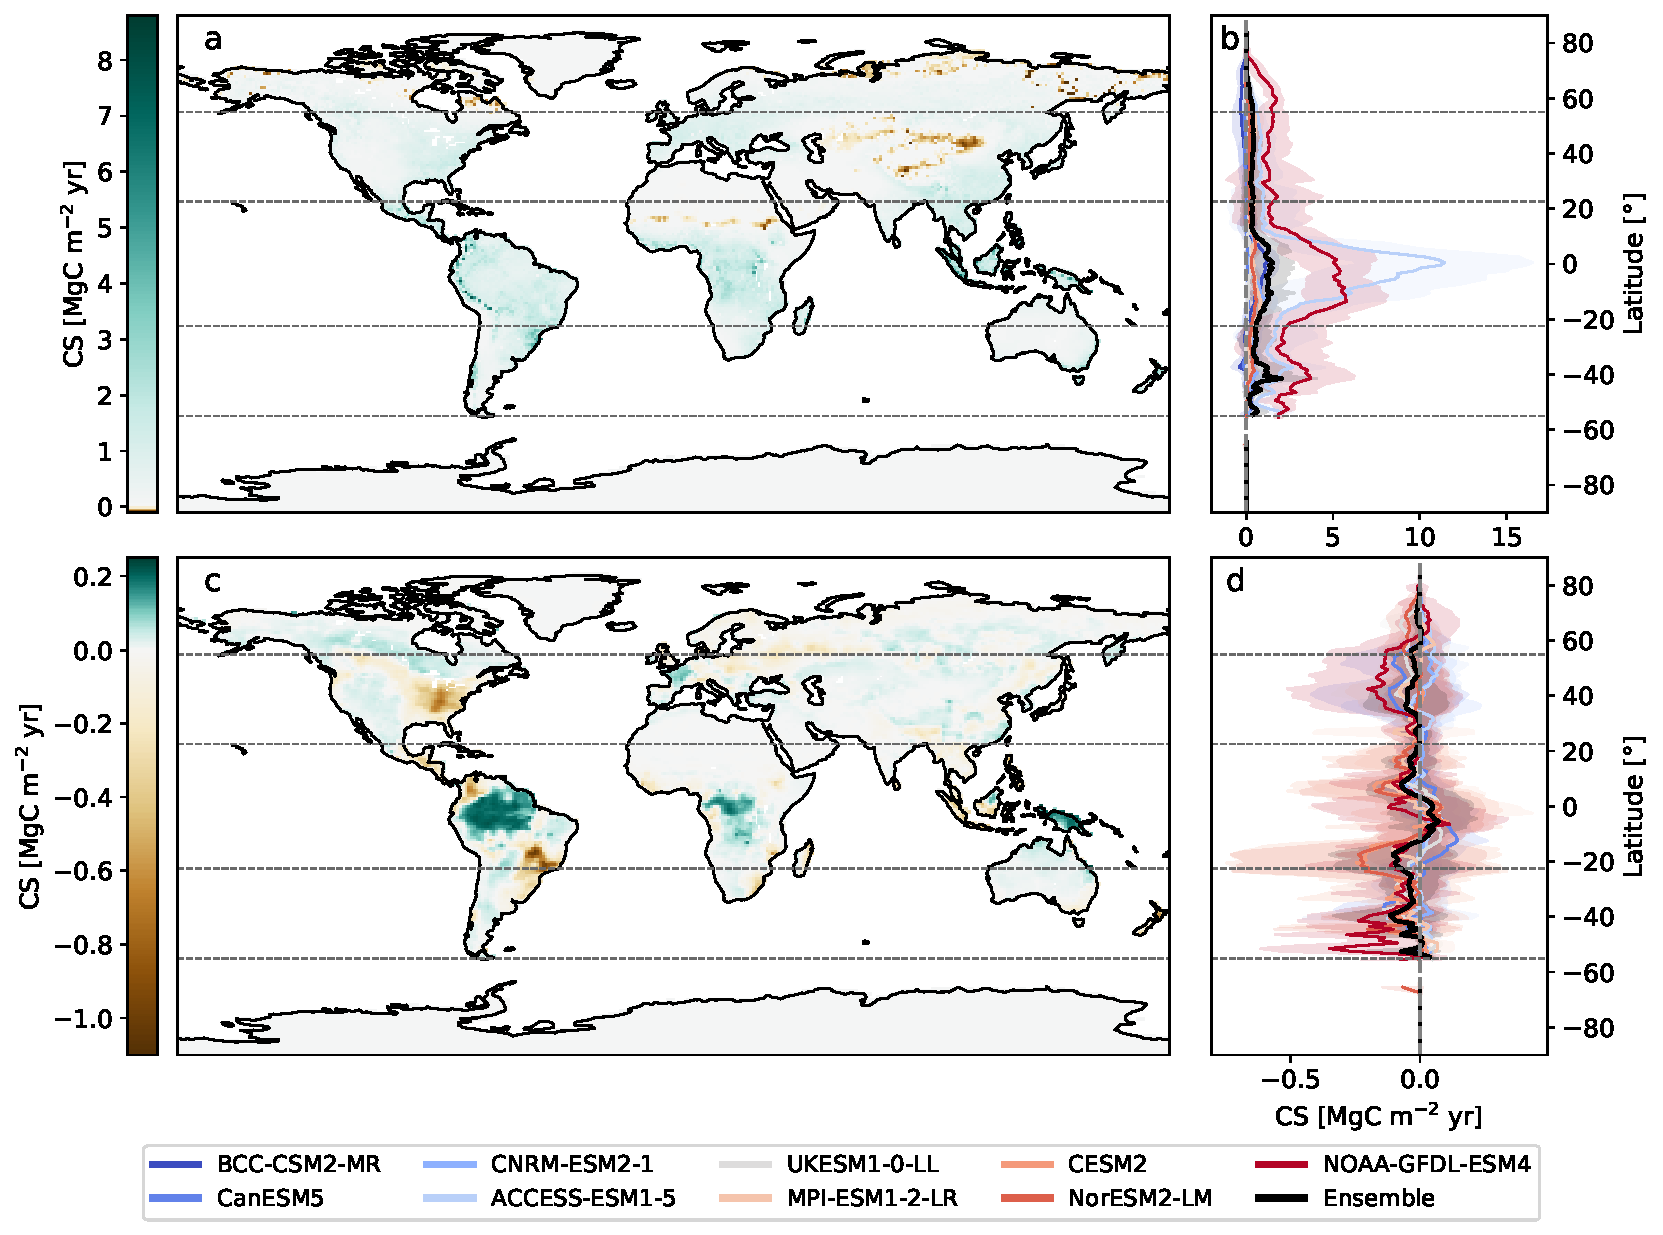
\includegraphics[width=11.4cm]{Figures/CMIP6_NEP_NBP_CS_map_latitude_mean.pdf}
    \caption{Carbon Sequestration (CS) spatial patterns based on NEP (a,b) and NBP (c,d) from CMIP6 models (1850-2014). a,c) Global distributions of CS based on the weighted ensemble average of 8 CMIP6 models, and b,d) latitudinal CS profiles for individual CMIP6 models (colored lines) and their ensemble average (black line). The vertical dashed lines in b and c represent null values of CS, and the shadow areas indicate two standard deviations from the spatial mean. Horizontal dotted lines define the latitudinal regions (tropics, mid latitudes, and high latitudes). Note that the color bar scales differ between panels a and c, as well as the scale of the x-axis in b and d.}
    \label{fig:CMIP6_NEP_NBP_map}
\end{SCfigure*}

CS across all latitudinal zones exhibits a consistent upward and increasing trend over time in all models, albeit with varying magnitudes. The NOAA-GFDL-ESM4 and ACCESS-ESM1-5 models show the highest CS values, while the CanESM5 and BCC-CSM2-MR models show the lowest (Fig.~\ref{fig:CMIP6_NEP_time}b and Fig.~S8). All models simulate that tropical regions retained the largest amount of carbon from 1850 to 2014, followed by mid-latitudes (Fig.~\ref{fig:CMIP6_NEP_time}). Although high latitudes sequester on average more carbon per unit area than mid-latitudes (Fig.~\ref{fig:CMIP6_NEP_NBP_map}b), the larger territorial expanse of mid-latitudes results in a higher total CS (Fig.~\ref{fig:CMIP6_NEP_time}). All CMIP6 models indicate positive CS values in the tropics throughout the studied period. In mid- and high-latitudes, at least one model (BCC-CSM2-MR) shows negative CS, where the accumulated balance between GPP and respiration leads to a net loss over the 165 years. Additionally, three models indicate nearly zero CS in high latitudes (Fig.~\ref{fig:CMIP6_NEP_time}b and Fig.~S8).

\begin{figure}%[\sidecaptionrelwidth][t!]
    \centering
    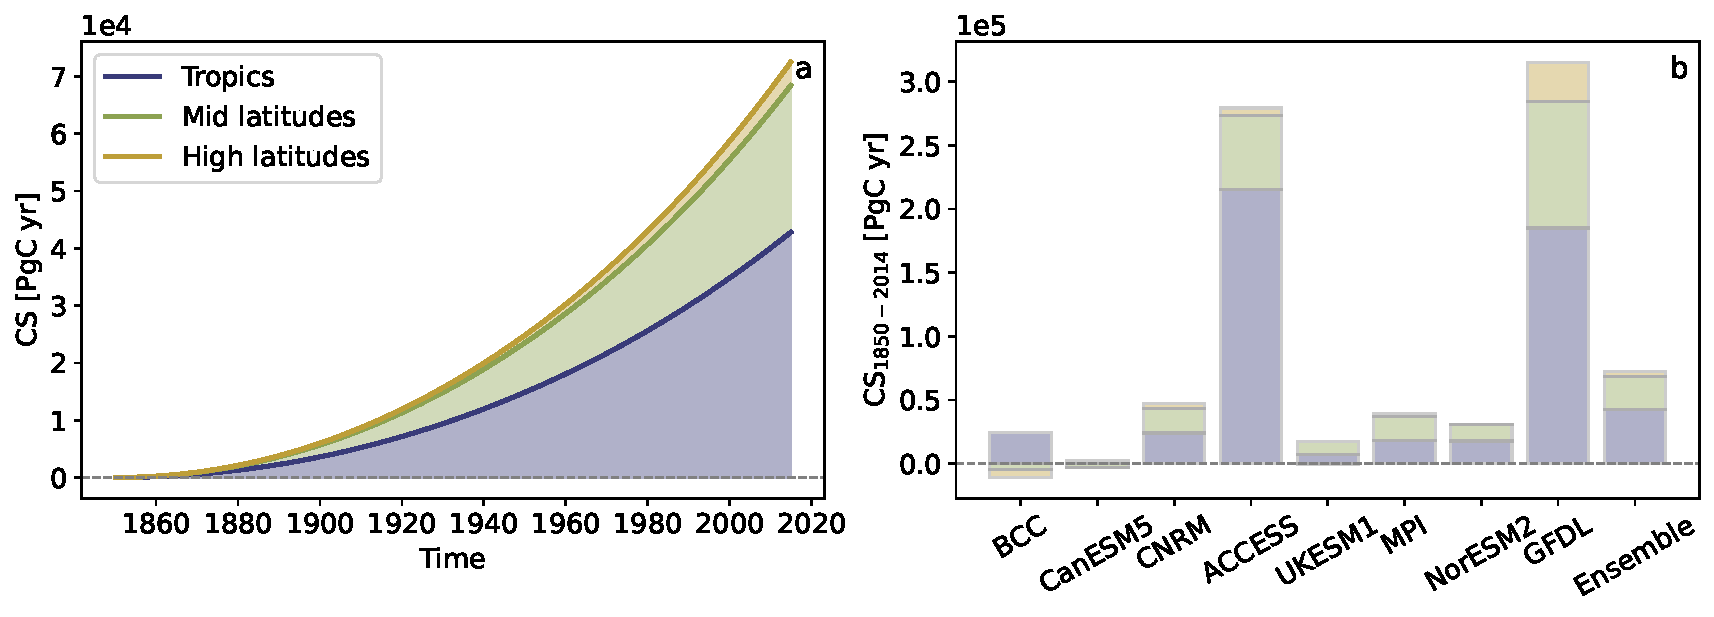
\includegraphics[width=1.0\linewidth]{Figures/CMIP6_NEP_CS_time_final_res.pdf}
    \caption{Temporal trends in Carbon Sequestration (CS) (a) and CS at the end of the period from 1850 to 2014 (b) calculated using NEP, and the contributions of latitudinal zones (colors). Panel a shows results from the CMIP6 models' average ensemble, and panel b shows results for each model alongside the ensemble. The dotted lines represent null CS values, with negative (positive) values indicating carbon debts (surpluses). To optimize space, only the initial part of each model name is displayed on the horizontal axes in b.}
    \label{fig:CMIP6_NEP_time}
\end{figure}

\subsection*{Disturbance impacts on Carbon Sequestration integrated over 165 years} 
The previous results, derived from the double integral of NEP, capture only the tradeoff between GPP and ecosystem respiration, excluding additional CO$_2$ emissions from disturbances like deforestation and fires. When calculating CS using the double integral of Net Biome Production (NBP)—which incorporates these additional disturbance emissions—spatial and temporal dynamics change markedly, with values about an order of magnitude smaller than those obtained with NEP (Figs.~\ref{fig:CMIP6_NEP_NBP_map}, \ref{fig:CMIP6_NEP_time}a and \ref{fig:CMIP6_NBP_time}a). These NBP-derived CS values are predominantly negative, reflecting a net carbon debt relative to pre-industrial stocks over the 165-year period, where cumulative losses exceed carbon gains. Globally accumulated CS is negative for all CMIP6 models except CNRM-ESM2-1 and ACCESS-ESM1-5, with the ensemble indicating a carbon debt of approximately 2800~PgC~yr for the period 1850-2014 (Fig.~\ref{fig:CMIP6_NBP_time}a). High-latitude regions show the least negative values, followed by the tropics (Fig.~\ref{fig:CMIP6_NBP_time}). Negative CS values are observed in 5 out of 8 models for the tropics, 6 for mid-latitudes, and 5 for high-latitudes (Fig.~\ref{fig:CMIP6_NBP_time}b and Fig.~S9). Unlike the monotonically increasing CS trend observed with NEP, the ensemble NBP-based CS trajectory shows an initial decline from 1850 to approximately 1970, followed by a modest recovery in recent decades (Fig.~\ref{fig:CMIP6_NBP_time}a).

The difference between CS calculated with NEP and NBP is dominated by tropical latitudes. Globally, the difference in CS between these two types of fluxes is approximately 75359~PgC~yr, with tropical regions accounting for 58\% (43722~PgC~yr) of this total (Table~S4). Therefore, fluxes excluded from NEP but included in NBP have a strong long-term effect on Carbon Sequestration, with these effects being particularly pronounced in tropical regions.

\begin{figure}
    \centering
    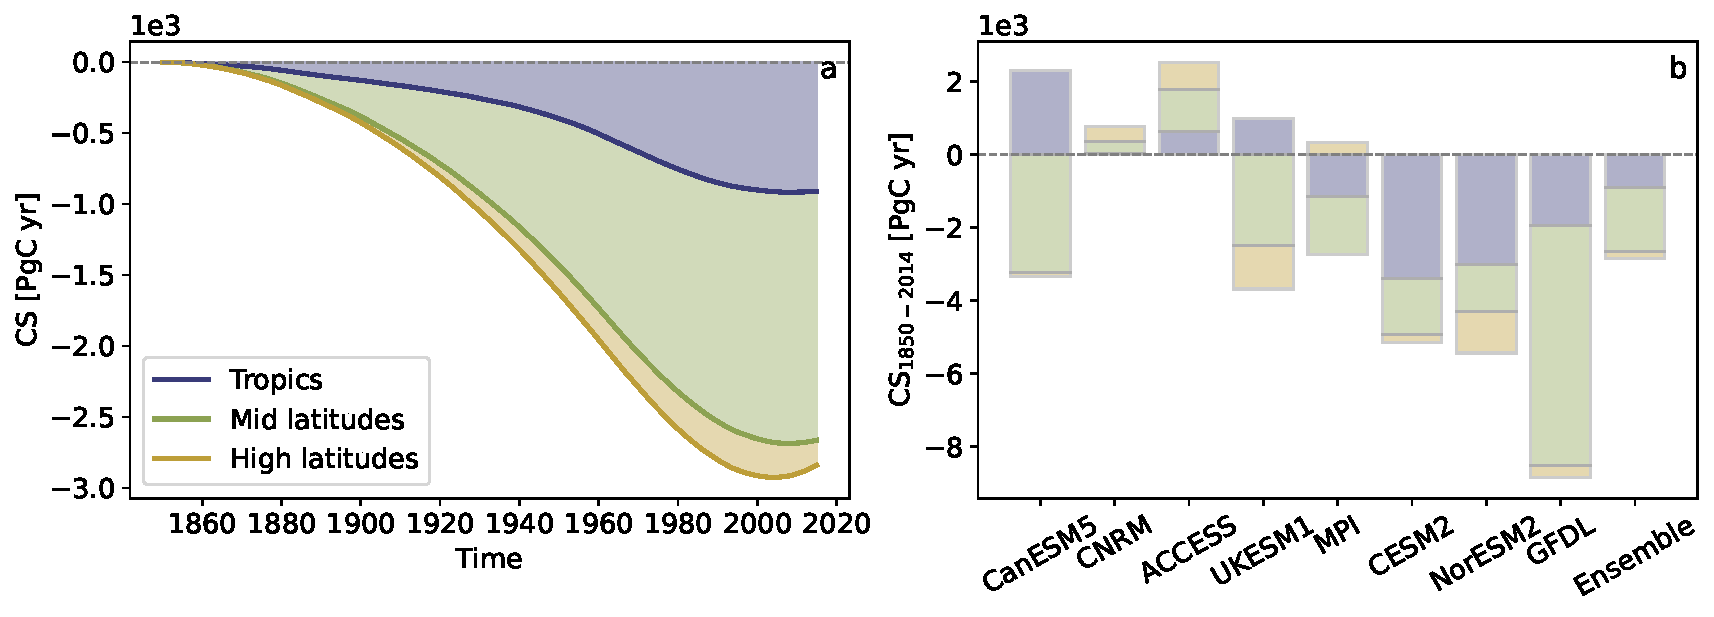
\includegraphics[width=1.0\linewidth]{Figures/CMIP6_NBP_CS_time_final_res.pdf}
    \caption{Temporal trends in Carbon Sequestration (CS) (a) and CS at the end of the period from 1850 to 2014 (b) calculated using NBP, and the contributions of latitudinal zones (colors). Panel a shows results from the CMIP6 models' average ensemble, and panel b shows results for each model alongside the ensemble. The dotted lines represent null CS values, with negative (positive) values indicating carbon debts (surpluses). To optimize space, only the initial part of each model name is displayed on the horizontal axes in b.}
    \label{fig:CMIP6_NBP_time}
\end{figure}

\subsection*{Comparison with TRENDY and observation-based products}
For the overlapping 14-year period (2001-2014), CS derived from NBP is substantially lower than NEP-based values across CMIP6, TRENDY, and observation-based products (Fig.~\ref{fig:Comparison_models}a,b). NEP-based CS from CMIP6, TRENDY, and X-BASE show tropical regions with the highest values and high latitudes with the lowest, aligning with previous results from 1850-2014 in Fig.~\ref{fig:CMIP6_NEP_time}. 
At the global scale, X-BASE provides CS values between CMIP6 and TRENDY, with lower values at mid-latitudes suggesting a slight overestimation of CS by the model ensembles. Although both ensemble models display similar latitudinal distributions of CS, CMIP6 consistently exceeds TRENDY by up to 250~PgC~yr globally (Fig.~\ref{fig:Comparison_models}a), despite not being fully independent, as some CMIP6 models use TRENDY vegetation models as their land component (Tables~S2 and S3).

When using NBP, CS remains predominantly positive across all products except for CAMS in tropical regions. In fact, CAMS produces the largest CS differences compared to CarboScope and the two model ensembles. CarboScope and CAMS products suggest an overestimation of CS by the two model ensembles in the tropics and underestimations in high latitudes (Fig.~\ref{fig:Comparison_models}b).
Mid-latitudes exhibit the highest NBP-based CS values during 2001-2014 (Fig.~\ref{fig:Comparison_models}b). The shift from negative CS values obtained with NBP over the longer 165-year period to positive values in the shorter 14-year period suggests that legacy effects of previous disturbances are not accounted for during the 2001-2014 period. This is particularly noticeable in the mid-latitude regions, where carbon recovery trends since the mid-20th century dominate the 14-year CS calculation, ignoring the historical disturbances. 

In tropical regions, the marked reduction from NEP-based to NBP-based CS during these 14 years is consistent across both model ensembles. CMIP6 models drop from 427~PgC~yr (NEP) to 33~PgC~yr (NBP) (394~PgC~yr difference), while TRENDY drops from 252~PgC~yr to 24~PgC~yr (228~PgC~yr difference) (Table~S4). This difference far exceeds that observed in other latitudes, driving the pronounced global differences between CS based on NEP versus NBP (Fig.~\ref{fig:Comparison_models}). 

\begin{figure}
    \centering
    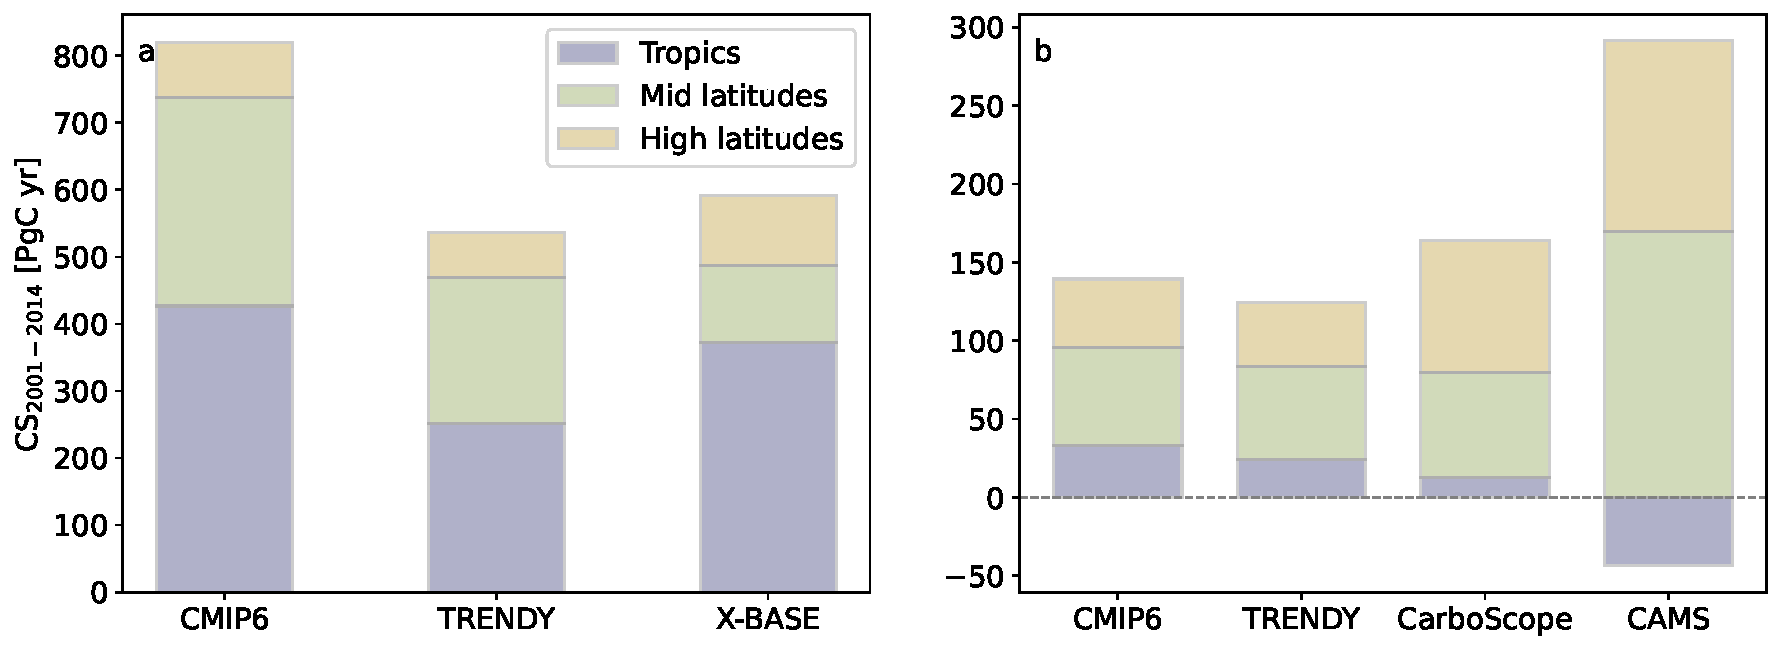
\includegraphics[width=1.0\linewidth]{Figures/Comparison_NEPvsNBP_res.pdf}
    \caption{Carbon sequestration (CS) across different products (2001-2014) calculated using NEP or NEE (a) and NBP (b) and contributions of latitudinal zones (colors). The dotted lines in a) indicate null values of CS. Negative (positive) values of CS indicate carbon debts (surplus). CMIP6 and TRENDY CS values correspond to the weighted ensemble of their respective models. Note that the y-axis of a) and b) do not have the same scale.}
    \label{fig:Comparison_models}
\end{figure}

\section*{Discussion}
\subsection*{Trade-off between high carbon assimilation and lagged respiratory responses}
Our approach to computing Carbon Sequestration (CS) as the double integral of carbon exchange between terrestrial ecosystems and the atmosphere enables the evaluation of long-term tradeoffs between carbon assimilation and lagged respiration responses. This approach implicitly incorporates the transit time of carbon through terrestrial ecosystems and quantifies the cumulative effects of the delayed release of carbon fluxes from ecosystems back to the atmosphere (see S1). A recent study using a similar methodology has demonstrated its applicability for analyzing long-term carbon dynamics \cite{Matthews2023}. Here, we found that high Carbon Sequestration arises from either high assimilation rates, as in tropical latitudes, or slow respiration responses, characteristic of high latitudes. However, the assimilation effect dominates globally over the lagged respiration effect. Therefore, the tropics emerged in our analysis as the region where more carbon can be retained longer, over decadal to centennial timescales, in the absence of disturbances. 

The monotonic increasing trend of NEP-based CS across all CMIP6 models is mostly the effect of larger GPP than respiration fluxes ($r_h+r_a$) for all regions during the entire simulation time-frame (Figs.~\ref{fig:CMIP6_NEP_time}a, \ref{fig:Comparison_models}a  and S1). Independently of whether this is an artifact of models or a real sustained carbon sink due to CO$_2$ and N fertilization, increased water use efficiency, or prolonged growing season \cite{Fernandez-Martinez2017,Fernandez-Martinez2019,OSullivan2019,Friedlingstein2023,Ruehr2023}, the key insight from our results is that as long as GPP monotonically increases, the lagged respiration response of the biosphere does not catch up, resulting in large quantities of carbon being retained over time in terrestrial ecosystems (and kept out of the atmosphere), as observed for CS calculated from NEP (Figs.~\ref{fig:CMIP6_NBP_time}, S1, S2, S8 and S12). However, this sustained monotonic increase in NEP-based CS does not yet account for additional losses such as fires, land-use change, and other emissions included in NBP that can completely change CS trajectories.


\subsection*{Consequences of disturbances}
Factors beyond climate, such as deforestation and fires, significantly reduce CS values. From 1850 to 2014, most CMIP6 models indicate cumulative carbon releases exceeded assimilation (Fig.~\ref{fig:CMIP6_NBP_time}), putting terrestrial ecosystems in a net carbon debt relative to pre-industrial carbon stocks. While the Amazon and Congo basins as well as Papua New Guinean forests still exhibit high positive CS values by the simulation's end period (Fig.~\ref{fig:CMIP6_NEP_NBP_map}c), mid- and high-latitude regions show substantial negative CS, leading to a large global-scale carbon debt (Fig.~\ref{fig:CMIP6_NBP_time}). This debt increased over time since the beginning of the industrial revolution (Fig.~\ref{fig:CMIP6_NBP_time}), mostly driven by large release fluxes in tropical and mid-latitude regions (Fig.~S1). However, after the 1970s, a recovery trajectory in CS indicates that the debt has been partially offset by forest regrowth in mid-latitudes. Despite this, the carbon debt remains significant by 2014, particularly in regions such as Eastern North America, Central America, the Northern Andes, and Eastern South America (Fig.~\ref{fig:CMIP6_NEP_NBP_map}c,d). 

Differences between NEP- and NBP-based CS highlight the critical role of disturbances on the biosphere's capacity to fix carbon out of the atmosphere and retain it for long periods (Figs.~\ref{fig:CMIP6_NEP_time} and ~\ref{fig:CMIP6_NBP_time}). These differences are particularly pronounced in the tropics, where high carbon fixation amounts are counteracted by substantial release fluxes from deforestation and other disturbances, hindering the ability of these regions to retain carbon over decadal timescales. Empirical studies report that respired carbon in tropical forests has a mean age in the order of a few years up to two decades \cite{Sierra2021JE,Chanca2025}. This implies that lagged respiration effects in the tropics are intrinsically rapid and can be exacerbated by additional losses due to disturbances, which would drastically reduce transit times. Consequently, when evaluated using the CS metric, the carbon loss over time in tropical regions significantly exceeds that of other latitudinal zones. 

When analyzing only the 2001-2014 period, CS calculated with NBP shifts to positive values, albeit remaining substantially lower than CS-based NEP for the same period (Fig.~\ref{fig:Comparison_models}). This shift in the trend of CS demonstrates how carbon flux balances can vary significantly depending on the chosen time horizon: over these 14 years, carbon inputs can offset recent losses. However, these short-term gains are insufficient to counteract the long-term accumulated historical carbon debts. 

\subsection*{Implications for climate-change mitigation policies}
The tradeoff between carbon assimilation and release over long timescales suggests that tropical regions play a critical role in assimilating and retaining carbon over time, but this capacity has been disrupted drastically by historical changes in land use, particularly deforestation \cite{Li2022}. This capacity also hints at the significant potential for increasing the carbon retention time in tropical regions through reduced disturbance levels and large-scale restoration of deforested areas. Such measures could repay a substantial share of the considerable terrestrial biosphere's carbon debt relative to pre-industrial global carbon stocks. Since the CS metric integrates both the amount of carbon and the time it is retained, it offers a robust framework for enhancing policies and programs aiming at carbon sequestration in natural systems, such as the Reducing Emissions from Deforestation and Forest Degradation in Developing Countries (REDD+) or other policies from the United Nations Framework Convention on Climate Change. CS increases as carbon is retained for longer times; therefore, it can be used to generate incentives for land management actions that promote the preservation of carbon storage over time. 

By incorporating the time component into carbon sequestration quantification, our analysis reveals the importance of explicitly defining temporal boundaries to assess the long-term carbon balance between the land and the atmosphere. Assessing Carbon Sequestration for recent and short integration times misses the importance of historical trends in carbon exchange. Human activity has disrupted the global carbon cycle mostly since the beginning of the Industrial Revolution, generating an important historical debt. Consequently, targets for global carbon-management policies must prioritize repaying this debt, as inaction will amplify its magnitude over time or allow for a very slow recovery, as seen during the last few decades.

Our analysis also suggests that terrestrial ecosystems can only act as significant and long-term (decades to centuries) sinks of anthropogenic carbon as long as assimilation increases monotonically over time, so lagged release effects do not have enough time to compensate for the increase in assimilation. However, this scenario seems unlikely for the future of the global carbon cycle, either because of a saturation effect of carbon assimilation resulting from multiple limitations \cite{Melnikova2021,Friedlingstein2023}, or because of an increase in the frequency and intensity of disturbances in terrestrial ecosystems \cite{Xu2021,Sitch2024}.

In summary, evidence from multiple models and observation-based products from the historical record of carbon exchange between the land and the atmosphere suggests that long-term global Carbon Sequestration is driven predominantly by the large assimilation fluxes in tropical regions, which dominate over their fast-release fluxes. However, the ability of the tropics to retain carbon over time has been disrupted dramatically since the beginning of the Industrial Revolution by land-use changes and fire regimes. At the same time, the tropics may be key to recovering the large global carbon debt accumulated since pre-industrial times. Incentives to recover this debt may be achieved by accounting for the time that carbon is preserved in natural ecosystems and remains out of the atmosphere, where it would contribute to radiative forcing. Overall, integrating time as a variable in carbon sequestration assessments can help us to effectively quantify tradeoffs between carbon assimilation and release, forecast timelines for historical carbon debt repayment under recovery scenarios, and better define policy instruments for climate change mitigation.


%very interesting from a CC mitigation perspective. Could we expect to ever pay that debt? How much C would we sequester if we pay it (how many degreesºC of increase less?)? Once payed, is there room to keep sequestering C beyond what we had in pre-industrial times?

\matmethods{
\subsection*{Datasets} We calculated Carbon Sequestration using numerical outputs of Net Ecosystem Production (NEP) (or Net Ecosystem Exchange, NEE) and Net Biome Production (NBP) from two model intercomparison products and three observation-based products (Figs.~S1-S3).


\subsubsection*{Model intercomparison products} 
We used the results of Gross Primary Production (GPP), autotrophic respiration (r$_a$), heterotrophic respiration (r$_h$), and Net Biome Production (NBP) from a set of Earth System Models (ESMs) participating in the most recent climate-carbon simulations under the sixth phase of the Coupled Model Intercomparison Project (CMIP6) \citep{Eyring2016}. Eight models provided monthly NBP output, while eight supplied data for the remaining variables of interest (BCC-CSM2-MR lacks NBP outputs, and CESM2 does not provide monthly GPP, $r_a$, and $r_h$) for the \emph{esm-hist} simulation (Table~S2). We used one ensemble member per model. The simulations span the period from 1850 to 2014 and are forced by prescribed anthropogenic CO$_2$ emissions rather than CO$_2$ concentrations. Data were sourced from The German Climate Computing Centre \hyperlink{https://cmip-data-pool.dkrz.de/CMIP6-Data-Pool.html}{DKRZ}. To enhance robustness, we also incorporated results from 20 Dynamic Global Vegetation Models (DGVMs) compiled by the TRENDY v13 project \citep{Sitch2024}, with 18 providing NBP outputs and all 20 supplying GPP, r$_a$, r$_h$ (Table~S3). We used experiment S3, which accounts for observed variations in atmospheric CO$_2$, land use change, and climate, and spans from 1700 to 2023. 

%Data were requested through the \hyperlink{https://globalcarbonbudgetdata.org/closed-access-requests.html}{Global Carbon Budget}. 

CMIP6 and TRENDY models were included in the analysis to leverage their complementary strengths.
TRENDY DGVMs focus on simulating terrestrial vegetation dynamics and ecosystem processes under actual historical climate conditions and land use, while CMIP6 ESMs provide a representation of the entire Earth system, including carbon-climate feedback, and often incorporating previous or current (sometimes simplified) versions of DGVMs used in TRENDY \citep{Argles2022,Weng2022}. For both CMIP6 and TRENDY models, NEP values are calculated as $\mathrm{NEP}=\mathrm{GPP}-(r_a+r_h)$.


% NBP: LPJml, DLEM, LPJ-GUESS only have annual data.
% rh: LPJ-GUESS does not have it. 
% CARDAMOM was removed to calculate the weights and the ensemble because it only has data from 2003.

\subsubsection*{Observation-based products}
We used results from two global atmospheric CO$_2$ inversion products: CarboScope and CAMS. These products estimate land-atmosphere net carbon exchange fluxes by combining CO$_2$ concentration measurements, atmospheric transport models, and information on anthropogenic carbon emission and land-atmosphere carbon exchange \citep{Kondo2022}. Specifically, we used the nbetEXToc\_v2024E version of \hyperlink{https://www.bgc-jena.mpg.de/CarboScope/?ID=nbetEXToc_v2024E}{CarboScope} \citep{Rodenbeck2005}, which provides daily flux estimates from 1957 to 2023 using measurements at 173 sites. For \hyperlink{https://ads.atmosphere.copernicus.eu/datasets/cams-global-greenhouse-gas-inversion?tab=overview}{CAMS} \citep{Chevallier2013}, we used version v24, which includes monthly data from 1979 to 2020 derived from over 100 surface measurement sites. The number of sites considered in these products has varied over time, with reported values reflecting the most recent simulations. Additionally, we incorporated Net Ecosystem Exchange (NEE) from \hyperlink{https://meta.icos-cp.eu/collections/zfwf1Ak2I7OlziGDTX8Xl6_T}{X-BASE} produced with FLUXCOM-X \citep{Nelson2024}. This machine-learning-based product is trained on in-situ eddy covariance and remote sensing data and provides monthly NEE estimates for the period 2001–2021.

In this study, we assumed that NEE and NEP are interchangeable since both represent the same underlying processes—GPP minus respiration—despite being calculated using different data sources. Note that X-BASE, CAMS, and CarboScope follow an atmospheric convention: negative values denote CO$_2$ uptake by ecosystems, whereas CMIP6 and TRENDY use the opposite sign convention (positive for net carbon assimilation).

% FLUXCOM-X: NEE (0.5°, monthly)  01/2001-12/2021
% CarboScope: NBP (2.5° x 2°, daily) 01/1957-12/2023
% CAMS: NBP (1.4° x 0.7°, monthly) 01/1979,12/2020

\subsection*{Homogenization and ensemble calculations}
To enable comparison, data from all products were regridded to a uniform $1^\circ\times1^\circ$ spatial resolution using the bilinear interpolation method implemented via \hyperlink{https://xesmf.readthedocs.io/}{xESMF \citep{zhuang2023}}. Datasets with higher temporal resolutions were standardized to monthly averages. CMIP6 calculations utilized the full-time series (1850-2014), while comparisons across products were restricted to their overlapping interval, i.e., 2001–2014. Positive NEP and NBP values were defined as fluxes moving from the atmosphere to the land surface, which contrasts with the conventions used in inverse models.

To calculate ensemble averages for CMIP6 and TRENDY models, we used a pixel-scale weighted averaging approach rather than a simple equal-weight average. This procedure, detailed in \cite{Sierra2025GMD}, assigns weights to each model based on its predictive performance against available data, following the multimodel inference framework presented by Burnham \& Anderson \cite{Burnham2002}, which builds on concepts developed by H. Akaike in the 1970s. The weighting procedure calculates each model's weight by measuring its distance from observed data, approximating the Kullback-Leibler distance between models and the unknown reality at the pixel scale. However, since we are dealing with global spatial models where direct observations are not available, we used data-driven products derived from sparse observations and scaled to the terrestrial surface. Specifically, we used X-BASE to assign model weights based on NEP, and CarboScope to assign weights for NBP averages (chosen for its longer time series compared to CAMS). The obtained static pixel weights are then applied to create time-dependent ensemble averages for CMIP6 and TRENDY models (Figs.~S4-S7).







%The calculation of weights ($w_i$) for each model $i$ is detailed in (\textcolor{red}{cite text with method}). Once $w_i$ are determined, the model ensemble ($\overline{x}$) is computed as
%\begin{equation}
%    \overline{x}=\sum_{i=1}^{k}w_i \cdot x_i
%\end{equation}
%where $k$ is the total number of models, and $x_i$ are the values of the variable of interest for model $i$. In this case, $x$ corresponds to NEP or NBP. 
 
% using all data from periods that overlap with the available data periods of CarboScope (CMIP6:1957-2014, TRENDY:1957-2023) or FLUXCOM-X (CMIP6:2001-2014, TRENDY:2001-2021) (\textcolor{red}{see Supplementary Figs.~1-4}).


% Units:
% CMIP6: kg m${-2}$ s${-1}$.
% TRENDY: kg m${-2}$ s${-1}$.
% FLUXCOM-X: g m${-2}$ d${-1}$.
% CarboScope: PgC yr${-1}$
% CAMS: g m${-2}$ s${-1}$.

\subsection*{Carbon sequestration} 
Carbon sequestration (CS) is defined here as the accumulated sequestration or loss of carbon in terrestrial ecosystems over time, which can be obtained as the integral of carbon storage over time \cite{Sierra2021}. This definition is equivalent to the double integral of the net carbon flux between the atmosphere and the terrestrial biosphere over a defined period starting at a reference year $t_0$ over a fixed time horizon $T$ \citep{Sierra2021,Metzler2024,Sierra2025}, as
\begin{equation} \label{eq:CS}
    \mbox{CS}\left(t_0,T\right):=\int^{t_0+T}_{t_0} \int^{t}_{t_0} \left[s(t')-r(t')\right]\mathrm{d}t'\mathrm{d}t,
\end{equation}
where $s(t')$ is the gross flux rate of carbon removed from the atmosphere at a given time $t'$, and $r(t')$ is the gross flux rate of carbon released from the terrestrial surface back to the atmosphere. This definition of CS accounts for both the fate of new carbon inputs and the legacy carbon already present in the system at $t_0$ \citep{Metzler2024}. It combines the amount of mass that enters the ecosystem with the time carbon remains stored (see Fig.~1 in Muñoz et al. \citep{Munoz2024}). In S1, we mathematically demonstrate that the CS definition in Eq.~\ref{eq:CS} implicitly accounts for the transit time of carbon in ecosystems, a very difficult metric to compute from observations or model output.

When calculating global Carbon Sequestration or aggregating it by latitudinal zones, the grid areas were factored into the computation, removing spatial units. Latitudinal zones are defined as tropical: 22.5$^\circ$S-22.5$^\circ$N, mid-latitudes: 22.5$^\circ$S-55.0$^\circ$S and 22.5$^\circ$N-55.0S$^\circ$N, and high latitudes: $>$55.0$^\circ$N.

\subsection*{Data and code availability} The codes used to produce the results shown in this article are archived on the repository under DOI: 10.5281/zenodo.15167573 \citep{Sierra2025}, as well as the result files.
}


\showmatmethods{} % Display the Materials and Methods section



\acknow{This project has received funding from the European Union’s Horizon 2020 research and innovation programme under the Marie SkłodowskaCurie grant agreement No 101110350 (DISEQ - The Drought Impact on the Climate Benefit of Carbon Sequestration). Additional funding has been provided by the Max Planck Society. M.F-M was supported by the European Research Council project ERC-StG-2022-101076740-STOIKOS and the Ramón y Cajal fellowship (RYC2021-031511-I) funded by the MICIU/AEI /10.13039/501100011033 and by FSE+. EK was supported by the ERTDF (JPMEERF24S12206) of the ERCA by MOE Japan. TN was supported by the German Federal Ministry of Education and Research (BMBF), project STEPSEC (Grant No. 01LS2102A). GH and LM were supported by NASA-CMS grants 80NSSC21K1059 and 80NSSC25K7221. We acknowledge the CMIP community for providing the climate model data, retained and globally distributed in the framework of the ESGF. The CMIP data of this study were replicated and made available for this study by the Deutsches Klimarechenzentrum (DKRZ). Also, we thank the developers of the CAMS, X-BASE, and the Jena CarboScope (C. Rödenbeck) products for publishing their results in an open platform.}% To generate the JSBACH TRENDYv13 data, resources of the DKRZ granted by its Scientific Steering Committee (WLA) under project ID bm1241 were used.}

\showacknow{} % Display the acknowledgments section


%\bibsplit[2]
%Use \bibsplit to split the references from the body of the text. Value "[2]" represents the number of reference in the left column (Note: Please avoid single column figures & tables on this page.)

% Bibliography
\subsection*{References}

%References should be cited in numerical order as they appear in text; this will be done automatically via bibtex, e.g. \cite{belkin2002using} and \cite{berard1994embedding,coifman2005geometric,phdthesis,masterthesis}. All references cited in the main text should be included in the main manuscript file.

\bibliography{biblio}

\end{document}


%\subsection*{Manuscript Length}

%A standard 6-page article is approximately 4,000 words, 50 references, and 4 medium-size graphical elements (i.e., figures and tables). The preferred length of articles remains at 6 pages, but PNAS will allow articles up to a maximum of 12 pages.




%PNAS must be able to archive the data essential to a published article. Where such archiving is not possible, deposition of data in public databases, such as GenBank, ArrayExpress, Protein Data Bank, Unidata, and others outlined in the \href{https://www.pnas.org/author-center/editorial-and-journal-policies#materials-and-data-availability}{Information for Authors}, is acceptable.

%\subsection*{Language-Editing Services}
%Prior to submission, authors who believe their manuscripts would benefit from professional editing are encouraged to use a language-editing service (see list at https://www.pnas.org/author-center/language-editing). PNAS does not take responsibility for or endorse these services, and their use has no bearing on acceptance of a manuscript for publication.

% \begin{figure}%[tbhp]
% \centering
% 
\includegraphics[width=.8\linewidth]{frog.pdf}
% \caption{Placeholder image of a frog with a long example legend to show justification setting.}
% \label{fig:frog}
% \end{figure}



% \begin{table}[t!]
% \centering
% \caption{Comparison of the fitted potential energy surfaces and ab initio benchmark electronic energy calculations}
% \begin{tabular}{lrrr}
% Species & CBS & CV & G3 \\
% \midrule
% 1. Acetaldehyde & 0.0 & 0.0 & 0.0 \\
% 2. Vinyl alcohol & 9.1 & 9.6 & 13.5 \\
% 3. Hydroxyethylidene & 50.8 & 51.2 & 54.0\\
% \bottomrule
% \end{tabular}

% \addtabletext{nomenclature for the TSs refers to the numbered species in the table.}
% \end{table}


% \subsection*{Digital Figures}

% EPS, high-resolution PDF, and PowerPoint are preferred formats for figures that will be used in the main manuscript. Authors may submit PRC or U3D files for 3D images; these must be accompanied by 2D representations in TIFF, EPS, or high-resolution PDF format. Color images must be in RGB (red, green, blue) mode. Include the font files for any text.

% Images must be provided at final size, preferably 1 column width (8.7cm). Figures wider than 1 column should be sized to 11.4cm or 17.8cm wide. Numbers, letters, and symbols should be no smaller than 6 points (2mm) and no larger than 12 points (6mm) after reduction and must be consistent.

% Figures and tables should be labelled and referenced in the standard way using the \verb|\label{}| and \verb|\ref{}| commands.

% Figure \ref{fig:frog} shows an example of how to insert a column-wide figure. To insert a figure wider than one column, please use the \verb|\begin{figure*}...\end{figure*}| environment. Figures wider than one column should be sized to 11.4 cm or 17.8 cm wide. Use \verb|\begin{SCfigure*}...\end{SCfigure*}| for a wide figure with side legends.

% \begin{SCfigure*}[\sidecaptionrelwidth][t!]
% \centering
% 
\includegraphics[width=11.4cm,height=11.4cm]{frog.pdf}
% \caption{This legend would be placed at the side of the figure, rather than below it.}\label{fig:side}
% \end{SCfigure*}


% \subsection*{Tables}
% Tables should be included in the main manuscript file and should not be uploaded separately.


% \subsection*{Single column equations}

% Authors may use 1- or 2-column equations in their article, according to their preference.

% To allow an equation to span both columns, use the \verb|\begin{figure*}...\end{figure*}| environment mentioned above for figures.

% Note that the use of the \verb|widetext| environment for equations is not recommended, and should not be used.

% \begin{figure*}[bt!]
% \begin{align*}
% (x+y)^3&=(x+y)(x+y)^2\\
%        &=(x+y)(x^2+2xy+y^2) \numberthis \label{eqn:example} \\
%        &=x^3+3x^2y+3xy^3+x^3.
% \end{align*}
% \end{figure*}



%\subsection*{Supporting Information Appendix (SI)}

% Authors should submit SI as a single separate SI Appendix PDF file, combining all text, figures, tables, movie legends, and SI references. SI will be published as provided by the authors; it will not be edited or composed. Additional details can be found in the \href{https://www.pnas.org/authors/submitting-your-manuscript#manuscript-formatting-guidelines}{PNAS Author Center}. The PNAS Overleaf SI template can be found \href{https://www.overleaf.com/latex/templates/pnas-template-for-supplementary-information/wqfsfqwyjtsd}{here}. Refer to the SI Appendix in the manuscript at an appropriate point in the text. Number supporting figures and tables starting with S1, S2, etc.

% Authors who place detailed materials and methods in an SI Appendix must provide sufficient detail in the main text methods to enable a reader to follow the logic of the procedures and results and also must reference the SI methods. If a paper is fundamentally a study of a new method or technique, then the methods must be described completely in the main text.

% \subsubsection*{SI Datasets}

% Supply .xlsx, .csv, .txt, .rtf, or .pdf files. This file type will be published in raw format and will not be edited or composed.


% \subsubsection*{SI Movies}

% Supply Audio Video Interleave (avi), Quicktime (mov), Windows Media (wmv), animated GIF (gif), or MPEG files. Movie legends should be included in the SI Appendix file. All movies should be submitted at the desired reproduction size and length. Movies should be no more than 10MB in size.


